\documentclass[svgnames,12pt,oneside, openright,a4paper]{scrbook}
\usepackage{tikz,blindtext} %%%% Usado para o titulo  de capitulos
\usepackage{palatino}
\usepackage{chngpage,calc}
\usepackage{hyperref}
\usepackage{kpfonts}
\usepackage{conf}
\usepackage[utf8]{inputenc}
\usepackage[portuguese, english, brazil]{babel} %%% Define o Idioma
\usepackage{setspace}
\usepackage{indentfirst}		% Indenta o primeiro parágrafo de cada seção.
\usepackage{color}				% Controle das cores
\usepackage{graphicx}			% Inclusão de gráficos
\usepackage{microtype} 			% para melhorias de justificação
\usepackage{transparent}
\usepackage{eso-pic}
\usepackage{float}
\usepackage{array}
\usepackage{epstopdf}
\usepackage{url}
\usepackage{multicol}
\usepackage{multirow}
\onehalfspacing
\newenvironment{palavraschaves}{\vspace{1cm}\textbf{Palavras Chaves: }}{}
\newenvironment{keywords}{\vspace{1cm}\textbf{Keywords: }}{}
%%%%%%%%%%%%%%%%%%%%%%%%%%%%Margens
\addtolength{\parindent}{-0.2cm}
\setlength{\textheight}{23cm}
\setlength{\textwidth}{15.5cm}
%%%%%%%%%%%%%%%%% Define o Titulo, o autor e o orientador%%%%%
\newcommand{\titulo}{Hipotireoidismo Por Amiodarona Em Paciente Com Doença De Chagas – Relato De Caso}
\newcommand{\orientador}{Prof. Dr. Roberto Kenji Nakamura Cuman}
\newcommand{\autor}{Gabrielle Rodrigues Munhoz\xspace}
\newcommand{\data}{Maringá 2017}
\newcommand{\membroa}{Prof . Dr . Roberto Kenji Nakamura Cuman $(Orientador)$}
\newcommand{\insta}{ Universidade Estadual de Maringá/DFA }
\newcommand{\membrob}{Profa . Dra . Gisleine Elisa Cavalcante da Silva }
\newcommand{\instb}{ Universidade Estadual de Maringá/DFA }
\newcommand{\membroc}{Prof. Me. Estela Louro }
\newcommand{\instc}{ Universidade Estadual de Maringá/DFA }
\usepackage{amssymb,amsmath,theorem}

%%%%%%Teoremas e outros Ambientes
%% TEOREMAS E OUTROS AMBIENTES

%%%%% TEOREMAS
\newtheorem{teo}{Teorema}[chapter]
\newtheorem{corol}[teo]{Corolário}
\newtheorem{ddefi}[teo]{Definição}
\newenvironment{definicao} % quadrado 
  {\begin{shaded} \begin{ddefi}\rm}{\end{ddefi} \end{shaded}}
\newenvironment{defi} % sem quadrado s
  {\begin{ddefi}\rm}{\end{ddefi}}
\newtheorem{prop}[teo]{Proposição}
\newtheorem{propri}[teo]{Propriedade}
\newtheorem{lema}[teo]{Lema}
\newtheorem{obss}[teo]{Observação}
\newtheorem{obss1}[teo]{Observações}
\newenvironment{obs}
  {\begin{obss}\rm}{\end{obss}}
  \newenvironment{observacoes}
  {\begin{obss1}\rm}{\end{obss1}}
\newtheorem{conj}[teo]{Conjectura}
%\newcounter{exemplocount}[chapter]
\newenvironment{exx}
  {\vspace{0.5cm} \refstepcounter{teo} \noindent  \textbf{Exemplo \arabic{chapter}.\arabic{teo}}}{\vspace{0.2cm} }
\newenvironment{ex}
  {\begin{exx}\rm}{\end{exx}}
\theorembodyfont{\rm}



% Demonstra��o (original hspace is 133mm)
\newenvironment{proof}[1][Demonstra\c{c}\~ao]{\noindent\textbf{#1:} }{\hfill $\Box$ }









\begin{document}

\newcommand{\universidade}{\protect{Universidade Estadual de Maringá}\xspace}
\newcommand{\lugar}{Maringá\xspace}
\begin{titlepage}

\changetext{}{}{}{0pt}{0pt}{}\null\vfill
 
\hspace{0.5cm}\begin{minipage}{\textwidth-1cm}
\begin{center}

\mbox{}\vspace{4cm}


{  \huge  \titulo } \\

\bigskip

{  \Large \bfseries \autor \\}



\end{center}

\vspace{5cm}

\begin{center}
 
\includegraphics[width=170px,keepaspectratio=true]{uemlogo.jpg} 
 % ufabc.: 0x0 pixel, -2147483648dpi, 0.00x0.00 cm, bb=
\end{center}
\end{minipage}

 
\begin{tikzpicture}
[remember picture,overlay]
    \node[yshift=-3cm] at (current page.north west)
      {\begin{tikzpicture}[remember picture, overlay]
        \draw[color=LightGray,fill=LightGray] (0,0) rectangle
          (\paperwidth,3cm);
        \node[anchor=east,xshift=1.01\paperwidth,rectangle,
              rounded corners=7pt,inner sep=11pt,
fill=Gray]              
%fill=MidnightBlue]
              {\color{white} \Large Trabalho de Conclusão de Curso -  Bacharelado em Farmácia};
       \end{tikzpicture}
      };
   \end{tikzpicture}
            
                           
\vfill
\end{titlepage}
\newpage
\vspace{4cm}

\begin{minipage}{12cm}
{  \Large \textbf{Título:} \titulo } \\

\bigskip

{  \large \textbf{Autor:}  \autor \\}
{\large \textbf{Orientador:}  \orientador
}

\bigskip

Projeto apresentado ao Departamento de Farmácia como requisito básico para a apresentação do Trabalho de Conclusão de Curso do Curso de Farmácia.

\end{minipage}
\vfill
\hspace{7cm}\begin{minipage}{9cm}
{\Large Banca Examinadora:}\vspace{0.4cm}

\textbf{\membroa}

\insta \vspace{0.4cm}

\textbf{\membrob}

\instb\vspace{0.4cm}

\textbf{\membroc}

\instc \vspace{0.4cm}

 Maringá, \data.
\end{minipage}












 

%%% Insere o Sum�rio
\pdfbookmark[0]{\contentsname}{toc}
\tableofcontents*
%%%%%%%%%%%%%%%%%
\chapter*{Agradecimento}

Agradeço a Deus, por ter me dado força, sabedoria, paciência e saúde para vencer os desafios diários. Obrigada pelas pessoas que colocou no meu caminho. 

Aos meus pais, que souberam confortar meu cansaço e dar estímulo quando mais precisei em toda a minha vida. Obrigada pelo amor, incentivo e esforço para realizar meus sonhos. Amo vocês. 

À minha irmã Nathalia pela alegria e carinho. Amo você. 

Agradeço a toda minha família, meus avós, tios, padrinhos e primos, pelos momentos de alegria e incentivo. 

Aos queridos e divertidos amigos da residência Lívia, Murillo, Monique, Vanessa, Indianathan, Natália, Talita, Gabriele, Naiara, Bruna e Fernanda pelos momentos de alegrias, angústias, apuros, ajuda e amizade. Foi muito bom conviver com vocês esses anos!

À professora e orientadora Gisleine pelos ensinamentos, dedicação, apoio, competência e amizade durante toda a realização da residência. Seus ensinamentos estarão presentes por toda a minha vida. 

Aos professores Estela, Silvana, Elza, Walderez, Jorge, Terezinha, Nelly e Roselania. Não tenho palavras para descrever a minha gratidão. 

A todos os colaboradores do Hospital Universitário de Maringá, em especial o Serviço de Farmácia Hospitalar, que sempre estavam dispostos a me auxiliar. 

À Maria dos Anjos por me mostrar que aquele que semeia bondade recebe amor. 

Aos preceptores que tive ao longo da residência pelo conhecimento transmitido, paciência e pelas contribuições para a minha vida profissional; 

Aos membros da banca, Dr. Donadio e Me. Simone por gentilmente aceitarem o convite e pelas contribuições. 

A todos que de qualquer forma colaboraram não só para que este trabalho pudesse ser realizado, como também para que eu me transformasse na pessoa que sou.


\chapter*{Resumo}

Uma reação adversa a medicamento $(RAM)$ é definida como $“$qualquer resposta prejudicial ou indesejável, não intencional, a um medicamento, que ocorre nas doses usualmente empregadas para profilaxia, diagnóstico ou terapia de doenças$“$. Apesar de incomum, existem casos de hipotireoidismo induzido pela Amiodarona. Este fármaco é um derivado diiodinado do benzofurano pertencente a classe III dos antiarrítmicos, sendo amplamente utilizada no tratamento de arritmias cardíacas comumente presentes em portadores da Doença de Chagas. O presente caso é proveniente do ambulatório de cardiologia de um hospital universitário do Paraná e referente a um paciente diagnosticado com Doença de Chagas e que apresentou uma disfunção tireoidiana precedida ao uso de Amiodarona. Após 14 meses em uso de 200mg de Amiodarona os exames de TSH e T4 livre demonstraram uma elevação nos níveis hormonais. Essas alterações foram rapidamente revertidas por meio da introdução do fármaco Puran T4. Por meio do Algoritmo de Naranjo pode-se classificar a Amiodarona como provável causadora do hipotireoidismo no paciente.  

\palavraschaves{Hipotireoidismo; Amiodarona; Reação Adversa a Medicamentos; Doença de Chagas;}

\chapter*{Abstract}
Versão em língua estrangeira do resumo. Obrigatório, pela ABNT. O título,  ABSTRACT, em inglês, RESUMEN, em espanhol castelhano...
Sugerimos Inglês.

\keywords{aubergine,carrot, radish} %%Palavras Chaves em Ingl�s
\chapter{Introdução}

De acordo com a Agência Nacional de Vigilância Sanitária $(ANVISA)$, uma reação adversa a medicamento $(RAM)$ é definida como $“$qualquer resposta prejudicial ou indesejável, não intencional, a um medicamento, que ocorre nas doses usualmente empregadas para profilaxia, diagnóstico ou terapia de doenças. No conceito de RAM pode-se observar a existência de uma relação causal entre o uso do medicamento e a ocorrência do problema.$”$.  
 
A Doença de Chagas, também chamada de Tripanossomíase Americana e até Tireoidite Parasitária pode se apresentar nas fases aguda na qual o paciente desenvolve febre, linfoadenopatia, edema palpebral unilateral, conhecido como sinal de Romana. Existe a fase intermediária da doença ou fase de latência que é quando o paciente fica assintomático, sendo apenas portador da moléstia, e esta pode se manter por vários anos. E por fim há a fase crônica, quando já ocorrem manifestações principalmente cardíacas $(SILVA, 2003)$. 

No que tange ao acometimento cardíaco, as arritmias ventriculares ocorrem comumente em pacientes chagásicos e os tipos são muito variados, desde extrassístoles ventriculares $(EV)$, taquicardias ventriculares sustentadas $(TVS)$, não sustentadas $(TVNS)$ e fibrilação ventricular $(FV)$. Geralmente os pacientes são acometidos por mais de um tipo de arritmia, o que piora o prognóstico $(RASSI Jr, 2012)$.

Neste contexto, para o tratamento das arritmias cardíacas a Amiodarona torna-se amplamente utilizada. Este fármaco antiarrítmico é considerado o mais eficaz e seguro, mesmo ocasionando muitos efeitos e toxicidade, principalmente pelo fato de interagir com os receptores nucleares dos hormônios tireoidianos, propiciando a ocorrência de hipotireoidismo $(GOODMAN, GILMAN, 2012)$. 

O hipotireoidismo como reação adversa ocorre pelo fato da amiodarona ser um derivado diiodinado do benzofurano, ou seja, possui dois átomos de iodo em sua estrutura que constituem 37$\%$ de sua massa, dos quais 10$\%$ são desiodados no corpo para a sua forma livre. Somando-se a isso, este fármaco possui uma grande semelhança estrutural com os hormônios tireoidianos, como a levotiroxina$(FIGURA 01) (PAVAN, JESUS, MACIEL, 2004)$.

\begin{figure}
\begin{center}

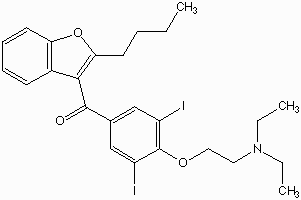
\includegraphics[scale=1]{molecula.jpg}

%\legend{Figura 01: molécula de amiodarona $(fonte: Micromedex® Solutions)$ }
\end{center}
\end{figure}

A alta quantidade de iodo na amiodarona é capaz de elevar a quantidade de iodo circulando pelo organismo e com isso há uma saturação da glândula tireoide, dessa maneira a produção dos hormônios tireoidianos T3 e T4 fica reduzida provisoriamente, enquanto que os níveis de TSH ficam aumentados, o que é denominado efeito Wolff-Chaikoff, que após algum tempo desaparece, levando a normalização do nível de TSH.$(MARQUES \& BUGALHO, 2011; FUKS, VAISMAN, BUESCU, 2002; LOPES, 2013)$. 

\chapter{Objetivos}

\begin{description}
   \item[a.] Geral
   
O trabalho em questão visa avaliar o hipotireoidismo como um efeito adverso ao uso crônico de amiodarona.    
   
   \item[b.] Específicos
   
- Verificar as manifestações clínicas do fármaco amiodarona; 

- Analisar a relação amiodarona x distúrbio tireoidiano;

- Observar a conduta do corpo clínico a cerca da doença desenvolvida;

- Analisar os exames realizados pelo paciente e a sua frequência; 

- Verificar se existem alternativas à amiodarona no mercado farmacêutico brasileiro; 
 
 \end{description}

\chapter{Metodologia}

Este trabalho foi desenvolvido em um hospital universitário do Paraná de acordo com a resolução 466/12 CNS/MS e deferida pelo Comitê Permanente de Ética em Pesquisa com Seres Humanos - COPEP da Universidade Estadual de Maringá, sob parecer aprovado em $n^{\circ}$. 1.760.441, em 04/10/2016.

Trata-se de um caso clínico proveniente do ambulatório de cardiologia do hospital em questão, referente a uma disfunção tireoidiana precedida ao uso de Amiodarona.

Foi utilizado o Algoritmo de Naranjo e colaboradores $($1981$)$ para estabelecer a relação de causalidade da reação adversa ao medicamento $($RAM$)$. Este algoritmo é constituído por dez perguntas, sendo que suas respostas são objetivas, havendo sempre duas opções de resposta $($sim ou não$)$, e visa obter informações a respeito das RAM, como pode ser observado na TABELA 1 $($CAPUCHO 2008$)$. 

A cada resposta pontos são atribuídos e ao final, por meio da somatória destes pontos, podem-se classificar as reações adversas em categorias de possibilidade como: definida, provável, possível, condicional ou duvidosa $(TABELA 2)$ $(CAPUCHO, 2008)$. 


Com relação aos medicamentos utilizados pelo paciente, analisou-se a possibilidade de haver interações medicamentosas, por meio do uso da base de dados Micromedex® Solutions como consta na TABELA 3. 

TABELA 3

\chapter{Relato de Caso}

Paciente J.R.S, sexo masculino, 76 anos, casado, ex-tabagista há 20 anos, refere ter hipertensão arterial sistêmica desde 2006, nega diabetes, e é portador de Chagas desde 2008.  

Em abril de 2010 inicia o uso de Amiodarona 200mg, devido ao fato de ter episódios intermitentes de Fibrilação Atrial.

Em janeiro de 2011, foi solicitado exame de TSH resultando em 68,239. 

Em junho de 2011 iniciou-se a suspeita de hipotireoidismo subclínico, sendo assim é realizada uma nova dosagem de TSH e T4 livre. T4 livre resultou 1,02 e o TSH 65,180. Com isso é prescrito Puran T4 50 microgramas por 15 dias e após esse período passaria a tomar 75microgramas. 

Em 17 de novembro de 2011 suspeitou-se de hipotireoidismo subclínico ou secundário à amiodarona, já que seu T4 livre estava 1,60 e seu TSH estava 2,990, ou seja, seu hipotireoidismo estava controlado. Então se solicitou um exame de Anticorpo Anti TPO para investigar. 

O exame Anti TPO deu 0,05, considerado negativo. 

Em Junho de 2012 seu T4 livre estava 1,39 e seu TSH 1,664. Um mês depois o T4 livre estava 10,44 e o TSH estava 2,450.

Em dezembro de 2012 seu TSH estava em 3,295.

Em março de 2013 o exame de TSH resultou em 1,442. 

Em maio de 2014, os exames resultaram em: TSH 2,427 e creatinina 1,23.

Em julho de 2015 no cardiologista, o paciente estava com seu TSH em 1,251. 

Em maio de 2016 o TSH estava em 4,0 e o clearance de creatinina em 53,39 ml/min/ 1,73m. 

Em janeiro de 2017 seu TSH apresentava-se 5,560 e o T4 livre estava 1,94, com isso a dose de puran T4 foi para 100microgramas. 

Em abril de 2017, seu TSH estava 2,26. 

\chapter{Avaliação de Causalidade}

TABELA 4

Por meio da aplicação ao Algoritmo de Naranjo $(1981)$, pode-se observar que o paciente possui uma reação adversa provável, sendo sua somatória igual a 6. Em casos de reações adversas com causalidade definida ou provável, o ideal é que essa RAM se torne prioridade para ações imediatas, podendo ocorrer a interdição de lotes de medicamentos, além da veiculação instantânea de alertas e a realização de notificações para a ANVISA $(CAPUCHO, 2008)$. 

No que tange às Reações Adversas a Medicamentos, como é o caso do hipotireoidismo induzido por amiodarona, é essencial que se realize a notificação, favorecendo assim o serviço de Farmacovigilância. De acordo com a Agência Nacional de Vigilância Sanitária, a Farmacovigilância pode ser definida como $“$a ciência e atividades relativas à identificação, avaliação, compreensão e prevenção de efeitos adversos ou quaisquer problemas relacionados ao uso de medicamentos$”$.

Dentre as funções da Farmacovigilância, pode-se citar a identificação, avaliação e monitoramento de ocorrências de eventos adversos referentes a utilização de medicamentos comercializados no mercado brasileiro, como forma de assegurar que os benefícios relacionados ao uso destes fármacos, sejam mais elevados do que seus próprios riscos $(ANVISA)$. 

\chapter{Acompanhamento Farmacoterapêutico}

TABELAS 5

\chapter{Discussão}

A Amiodarona é um medicamento antiarrítmico que faz parte da classe III. Nos dias atuais, consiste em um dos fármacos mais usados no que tange a manutenção do ritmo sinusal em doentes com fibrilação atrial ou flutter atrial, e recentemente foi incorporada as diretivas da American Heart Association como um dos medicamentos utilizados na paragem cardíaca $(LIMA et al, 2012)$. 

O hipotireoidismo ocorre de maneira mais comum em mulheres, indivíduos de idades mais avançadas, e pacientes com história passada de Tireoidite de Hashimoto $(LIMA et al, 2012)$. Ainda, o risco de ocorrer hipotireoidismo é de cerca de 7$\%$ se a paciente for do sexo feminino ou apresentar anticorpos antitireoperoxidase $(Anti-TPO)$ positivo, mas esse risco se eleva para 13.5$\%$ caso a paciente seja mulher e tenha Anti-TPO positivo também $(URSELLA et al, 2005; NARAYANA, WOODS, BOOS, 2011)$.   

Sabe-se que o nível de iodo do ambiente pode propiciar a ocorrência de distúrbios de tireoide, por exemplo, em localidades aonde a taxa de iodo é menor os casos de hipertireoidismo são mais comuns. De forma diferente, o hipotireoidismo se torna mais comum em localidades aonde a taxa de iodo no ambiente é suficiente $(ROSS, et al, 2005 ;NARAYANA, WOODS, BOOS, 2011; LIMA et al, 2012)$. 

De acordo com Lima et al $(2012)$, o hipotireoidismo desenvolve-se nos primeiros 18 meses de tratamento com a amiodarona, sendo compatível com o paciente em estudo, uma vez que seu quadro de hipotireoidismo foi diagnosticado em 14 meses, sendo iniciada a sua terapia com levotiroxina. 

Um método comumente utilizado para auxiliar na decisão terapêutica sobre a autoimunidade tireoidiana é o teste de dosagem de anticorpos tireoperoxidase $(Anti-TPO)$ $(GHETTI, 2014)$, sendo que estes estão mais presentes na população idosa $(SILVA, 2013)$. 

A Tireoperoxidase $(TPO)$ é uma glicoproteína encontrada na borda apical das células foliculares da tireoide, estando envolvida na formação dos hormônios tireoidianos. Ela possui função catalítica, sendo capaz de realizar a iodação e acoplamento de resíduos da molécula da tireoglobulina, originando então os hormônios da tireoide $(KASAMATSU, MACIEL, VIEIRA, 2001)$. 

E a principal causa de Hipotireoidismo Subclínico é o fato de o paciente apresentar tireoidite autoimune, com isso, seus níveis de TSH se tornam muito elevados, enquanto que os níveis de T4 se mantêm normais $(GHETTI, 2014)$. 

Mesmo que as alterações nos níveis de TSH sejam brandas no hipotireoidismo após o início do tratamento farmacoterapêutico com Amiodarona, o diagnóstico em si associa os valores de TSH elevados $(>10mU/l)$ com os valores normais ou baixos de T4 livre. Níveis baixos de T3 e T3 livre são indícios menos confiáveis de hipotireoidismo, uma vez que podem ocorrem em pacientes eutiroideos que simplesmente fazem uso de amiodarona, pois esta é capaz de reduzir a conversão de T4 em T3 $(NARAYANA, WOODS, BOOS, 2011)$. 

O paciente em estudo faz uso de Amiodarona há 7 anos. No início desta terapia foi observado um desequilíbrio do nível hormonal de TSH e T4 livre, pois até o momento o paciente era considerado eutiroideo. Exames foram realizados para que houvesse um acompanhamento de seus níveis hormonais, porém o desequilíbrio se manteve, e com isso iniciou-se o tratamento com a levotiroxina. 

O ideal é que haja o uso de levotiroxina, porém geralmente as dosagens são mais altas do que as usadas normalmente em pacientes com hipotireoidismo convencional, além disso, prioriza-se por tentar manter a amiodarona $(LIMA et al, 2012)$.

De acordo com Ursella et al $(2005)$, após 3 meses de uso de Amiodarona, atinge-se o steady state e além disso, o T4 livre e o total, se mantém dentro da normalidade, ou até levemente elevados. Em detrimento, o TSH sérico retorna aos níveis normais após cerca de 12 semanas de terapia. Pode-se dizer que a normalização do TSH é devido ao aumento na produção de T4, além do escape do efeito de Wolff-Chaikoff que supera o impedimento na produção de T3 e com isso eleva seus níveis séricos.

Com relação ao paciente analisado, pode-se observar no GRÁFICO 1 que os níveis de hormônio TSH e T4 livre do paciente em estudo foram se alterando até atingirem uma taxa considerada normal. O paciente iniciou o uso de amiodarona no ano de 2010, e em janeiro de 2011 foi feita a primeira dosagem de TSH e T4 constatando que ambos estavam alterados, porém ao longo dos meses a dosagem de T4 livre foi minimamente solicitada por parte dos médicos, por esse motivo o gráfico encontra-se com tão poucos dados. Contudo, apesar da baixa quantidade de informações sabe-se que paciente possui cardiopatias severas, sendo mais vulnerável aos efeitos dos hormônios tireoidianos, como a elevação no consumo de oxigênio, e assim, a dosagem de levotiroxina $(Puran T4)$ deve ser prescrita para que o hormônio TSH seja mantido na metade superior considerada normal $(RAMOS-DIAS, SENGER, 2011)$.

Com relação ao paciente analisado, pode-se observar no GRÁFICO 1 que os níveis de hormônio TSH e T4 livre do paciente em estudo foram se alterando até atingirem uma taxa considerada normal. O paciente iniciou o uso de amiodarona no ano de 2010, e em janeiro de 2011 foi feita a primeira dosagem de TSH e T4 constatando que ambos estavam alterados, porém ao longo dos meses a dosagem de T4 livre foi minimamente solicitada por parte dos médicos, por esse motivo o gráfico encontra-se com tão poucos dados. Contudo, apesar da baixa quantidade de informações sabe-se que paciente possui cardiopatias severas, sendo mais vulnerável aos efeitos dos hormônios tireoidianos, como a elevação no consumo de oxigênio, e assim, a dosagem de levotiroxina $(Puran T4)$ deve ser prescrita para que o hormônio TSH seja mantido na metade superior considerada normal $(RAMOS-DIAS, SENGER, 2011)$.

O uso crônico da amiodarona tem propiciado muitos estudos para o desenvolvimento de novos fármacos que sejam mais seguros, que possam ser capaz de substituí-la, porém mantendo o ritmo sinusal adequado ao longo prazo na fibrilação atrial. Dessa maneira um fármaco que vinha ganhando destaque era a dronedarona, descoberto e desenvolvido pela Sanofi-Aventis $(FIGURA 3)$.

\begin{figure}
\begin{center}

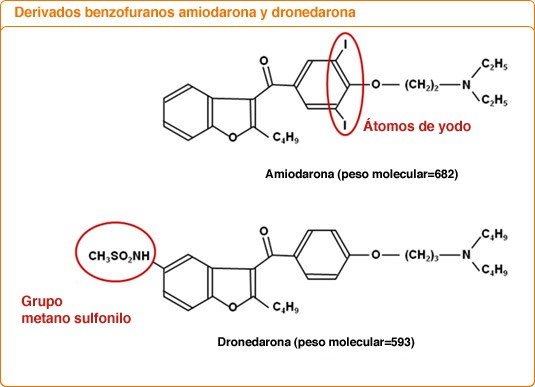
\includegraphics[scale=1]{molecula2.jpg}

%\legend{Figura 01: molécula de amiodarona $(fonte: Micromedex® Solutions)$ }
\end{center}
\end{figure}

A dronedarona $(Multaq)$ é também um derivado benzofurânico, porém não é iodado, o que evitaria o acúmulo excessivo de iodo no organismo $(LOPES, 2013)$. $“$Foi desenvolvida para pacientes adultos, clinicamente estáveis, com história de Fibrilação atrial $(FA)$ ou episódio recente de FA não permanente, para evirar a recorrência de FA ou reduzir a frequência ventricular$”$ $(SANOFI-AVENTIS, 2009)$. 

Tanto a amiodarona, quanto a dronedarona estão disponíveis no Sistema Único de Saúde $(SUS)$, sendo que está última foi incluída na $“Lista Positiva”$ em 2014 pelo Governo Federal, por meio do decreto n$\circ$ 8.271, com mais 173 outros medicamentos. 

A questão central é o fato de a equipe médica optar pela manutenção da Amiodarona, mesmo dispondo de uma alternativa. Pode-se dizer que há um risco benefício mantendo-se a Amiodarona, porque mesmo que ocasione efeitos adversos relacionados a glândula tireoide levando a transtornos ao paciente, ela é capaz de manter o ritmo sinusal dentro dos limites normais. Entretanto no caso da dronedarona, os estudos foram positivos apenas inicialmente, uma vez que seu uso teria de ser limitado apenas para pacientes cuja insuficiência cardíaca fosse de caráter leve, do contrário, as chances de hospitalização ou até piora no quadro do paciente poderiam se elevar $(LOPES, 2013; FDA, 2011; SANOFI-AVENTIS, 2009)$.  

A agência federal americana do Departamento de Saúde e Serviços Humanos dos Estados Unidos $(FDA)$ fez um alerta tanto os profissionais de saúde, quanto aos pacientes em uso do fármaco dronedarona $(multaq)$, que este poderia causar danos hepáticos raros, porém de alta gravidade. Foram relatados dois casos de pacientes que foram submetidos a transplantes hepáticos depois de fazer tratamento com este medicamento.  Em ambos os casos as pacientes eram do sexo feminino e possuíam cerca de 70 anos. A primeira paciente fez uso da dronedarona por 4 meses e meio devido a fibrilação atrial intermitente, hipertensão arterial e doença coronariana. Duas semanas antes de ser hospitalizada ela mencionou estar sentindo um grande cansaço. Uma semana antes da sua admissão hospitalar, ela abandonou a terapia com Multaq e assim que deu entrada no hospital notou-se que ela estava com icterícia, coagulopatia e hiperbilirrubinemia, que progrediu rapidamente para encefalopatia hepática. O tratamento pré-transplante não evidenciou nenhuma outra etiologia para a falência hepática. A segunda paciente possuía uma história médica de fibrilação atrial paroxística e Síndrome de Sjogren, e dessa maneira fez um tratamento de cerca de seis meses com dronedarona. Entretanto nesse prazo ela começou a desenvolver fraqueza, dor abdominal, coagulopatia e hiperbilirrubinemia. Um mês depois foi realizado o seu transplante. Em ambos os casos a análise posterior do fígado evidenciou extensivas necroses hepatocelulares $(FDA, 2011)$.

Avaliar a causalidade é um fator essencial no que tange à análise das reações adversas, designando uma relação entre o fármaco e o quadro suspeito. Contudo, se torna árduo estabelecer se o quadro sintomático realmente pode ser decorrente de um fármaco ou não. Diagnosticar uma reação adversa é como uma demonstração de disgnóstico diferencial, no qual o elemento problemático é uma droga intrinsecamente utilizada para curar $(MENEZES \& CHINCILLA, 2011)$. 

As reações adversas relacionadas ao consumo de medicamentos seja Amiodarona ou Dronedarona podem ser classificadas de acordo com vários tipos de algoritmos, como de Karch e Lasagna, além do também conhecido algoritmo de Naranjo. Este último é amplamente utilizado devido ao seu fácil manuseio e entendimento $(HEBERLE, 2009)$.

O algoritmo de Naranjo se baseia numa escala de probabilidade incluindo uma sequência cronológica desde a administração do medicamento no paciente até o aparecimento do quadro clínico $($considerando a descrição preliminar da reação adversa contida na literatura médica, ou as propriedades farmacológicas do medicamento$)$. Ainda, este algoritmo analisa se a reação adversa se mantém ou não após a retirada do medicamento suspeito ou o uso de um placebo, e a existência de novas possibilidades farmacoterapeuticas $(OPAS, 2011)$.  

A observação por meio do algoritmo de Naranjo possibilita que as reações adversas $(RAM)$ sejam classificadas em categorias $(VARALLO, 2010)$: 

\begin{enumerate}

\item[1.] Definida: é um caso clínico, que pode incluir anormalidades em exames laboratoriais, que ocorram em um espaço de tempo relevante no que diz respeito à administração do medicamento suspeito, e que, além disso, não possa ser justificado por alguma doença ou por outros medicamentos e substâncias.  O resultado com a retirada do medicamento deve ser clinicamente plausível. 

\item[2.] Provável: evento clínico, que pode integrar anormalidades em exames laboratoriais, com um intervalo temporal razoável da administração do medicamento, havendo uma impossibilidade de ser incumbido a outra moléstia ou substância. Não é preciso haver reintrodução para finalizar a definição. 

\item[3.] Possível: evento clínico que pode incluir alterações laboratoriais havendo um tempo razoável da administração do medicamento, mas que poderia ser justificado por alguma doença concomitante, ou outros medicamentos.

\item[4.] Duvidosa: evento clínico que pode incluir alterações nos exames laboratoriais, que apresentam uma relação temporal com o uso do medicamento que torna improvável a relação de causa e no qual outro medicamento ou substância propicia explicações plausíveis.

\end{enumerate}
   

%%%%%%%%%%%%%%%%%%%BIbliografia


\end{document}
